\newpage
\subsection{Convolutional layers}
\begin{wrapfigure}{r}{0.3\linewidth}
	\vspace{-1.2cm}
	\centering
	\begin{subfigure}[b]{\linewidth}
		\centering
		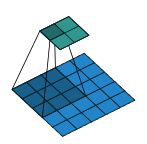
\includegraphics[width=0.6\linewidth]{Materials/Theory/convolution}
		\caption{Convolution of a 5x5 input image with a 3x3 kernel using no padding and 1 stride, producing a 2x2 output image.}
		\label{convolution}
	\end{subfigure}
	\\
	\begin{subfigure}[b]{\linewidth}
		\centering
		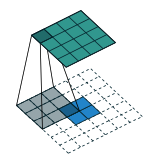
\includegraphics[width=0.6\linewidth]{Materials/Theory/transposedconv}
		\caption{Transposed convolution of a 2x2 input image with a 3x3 kernel using 2 'layers' of padding all around and 1 stride, producing a 4x4 output image.}
		\label{transposedconv}
	\end{subfigure}
	\caption{Examples of a convolution and a transposed convolution. Blue layer denotes input image, cyan layer denotes output image, shaded squares denotes kernel and dotted squares denotes padding. Images are from \cite{convolutionarticle}.}
\end{wrapfigure}
In the convolution layers a (discrete) convolution is performed. A (discrete) convolution is an operation in which a kernel is moved over a signal and the output is the sum of products between the kernel and the overlapping elements. In our concrete case we are dealing with images, which can be thought of as an array of pixel values. If we simplify the discussion to greyscale images, we simply have an array of same dimension as the image filled with pixel intensities. We can now overlay the input image with our kernel and compute the sum of products. We can now move the kernel over the image, and each time we move the kernel we get an output. The number of pixels we move the kernel is called the \textit{stride}. After having moved the kernel over the entire image, the output is a new image which dimensions are smaller than the input. How much smaller depends on the stride and the kernel size. If a certain output dimension is needed after a convolution, the input images might need to be padded with 'extra' pixels. Several strategies exists for padding, the most common is to pad with zeros. An illustration of a convolution can be seen in \autoref{convolution} \cite{convolutionarticle}.

\subsection{Max pooling layers}
In the max pooling layers a kernel is defined and moved around the input image. The output is then the largest value inside the kernel. The number of pixels it is moved is again determined by a stride. A max pooling layer using a 2x2 kernel and a stride of 2 thus halves both input image dimensions as a 2x2 area in the input image becomes a single pixel in the output image \cite{convolutionarticle}.

\subsection{Transposed convolutions}
In the upsampling layers we want to perform a 'reversed' convolution where we go from a small image to a larger image while still keeping the connectivity pattern. The 'up-conv' layer used in \autoref{unet} is also called a \textit{transposed convolution}, and we perform these instead of simply upscaling the image because we can learn an optimal way of upscaling the images. To perform a transposed convolution we compute the output shape of a convolution with a given input shape and then we invert the input and output shapes. The input would then be padded with zeroes to comply with the kernel size. As an example we would like to perform a convolution with a 3x3 kernel on a 4x4 input image with no padding and 1 stride. This would produce a 2x2 output image. Inverting the input and output, we would then have to convolve a 2x2 image with a 3x3 kernel to get a 4x4 output. As the 2x2 image does not comply with the 3x3 kernel, we pad it with 2 'layers' of zeroes all around. An illustration of a transposed convolution can be seen in \autoref{transposedconv}. Although this is not the most efficient way of performing a transposed convolution, it gives an intuition of what is happening \cite{convolutionarticle}.

\subsection{Convolutional Neural Networks}
\begin{wrapfigure}{l}{0.6\linewidth}
	\centering
	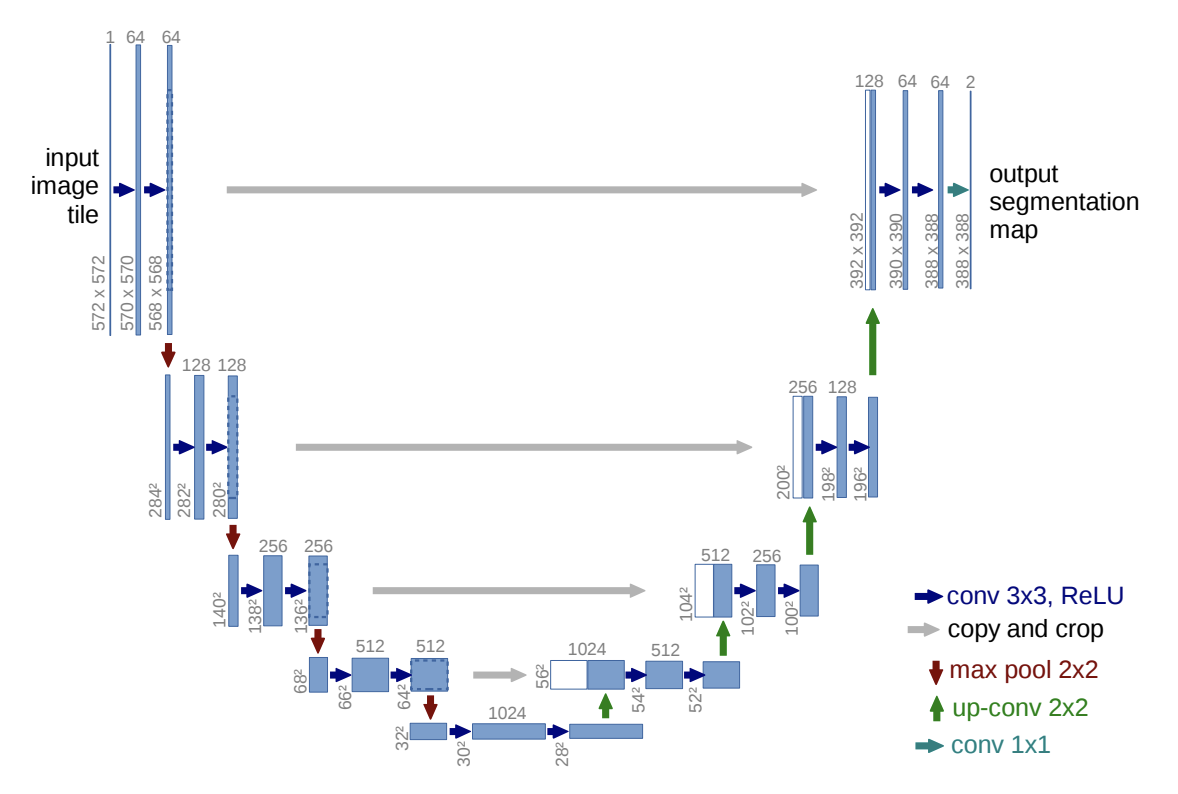
\includegraphics[width=\linewidth]{Materials/Theory/unet}
	\caption{U-Net architecture example for input image of size 572x572 pixels. Image taken from \cite{unetarticle}}
	\label{unet}
\end{wrapfigure}
Deep neural networks (DNN's) are neural networks with several layers between the input and the output which allows them to learn complex non-linear relationships in the data. Each layer holds a number of neurons which usually are fully connected, meaning each output from the neurons in the previous layer goes into the neurons of the next layer. DNN's have a lot of parameters which are getting trained as each neuron have their own weight. A convolutional neural network (CNN) is a special class of DNN's which mainly uses convolutional layers. This makes it possible to process images as it is the weights of a kernel which are trained rather than processing each individual pixel in the images. CNN's are usually used for image segmentation or in general tasks which requires processing of images. A concrete example of a CNN could be a modified U-Net model where the encoder is replaced by a ResNet-18 model. The original U-Net architecture can be seen in \autoref{unet}.\\
The U-Net architecture can be split in two parts, a left part which downscales the processed image and a right half which upscales the image again. Replacing the encoder of the U-Net model means this left part is replaced with the ResNet-18 model. ResNet-18 begins by performing a 7x7 convolution with a stride of two followed by a 3x3 max pooling with a stride of two. It then follows a pattern of doing two 3x3 convolutions each followed by a rectified linear unit operation before a skip connection, skipping two convolutions. After three convolutions the fourth uses a stride of two to downsample the image. This results in the feature map getting halved in size and the number of the feature channels getting doubled after each downsampling step. Three downsamplings are done this way before we reach the right half of the U-Net model \cite{resnet}. For the right half, an upsampling followed by a 2x2 convolution is performed. This halves the number of feature channels and doubles the size of the feature map. Then a concatenation from the corresponding left half feature map is done. These skips (along with whose in the ResNet-18 model) allows the model to recover lost spatial information and alleviates the vanishing gradient problem, which results in improved performance. After the skips, two 3x3 convolutions are performed each followed by a rectified linear unit operation. In the end a 1x1 convolution is performed to map the final feature map to the correct number of prediction classes \cite{unetarticle}. Another example of a CNN is LinkNet which in a similar fashion as to U-Net has a left part which downsamples images and a right path which then upsamples them with skip connection in between, but instead of concatenating the feature maps after these skips, in LinkNet they are added. This reduces the number of parameters the network needs to learn \cite{linknet}.\\
The clear advantages of CNN's are how accurate and how fast the models can make predictions. This allows for fast automatisation of suited tasks. However, it might take weeks to train state of the art models without any guarantees if it will perform better than its predecessor, and so it is a time consuming process to develop good models. It is also taxing on power consumption and the environment to train for these long periods of time. Often times the most limiting factor in model development is gathering varied data or annotating this data.

\subsection{Transfer learning}
Transfer learning is a common technique where a model developed for some task is reused as starting point for another model. This allows the model to get a 'head start' as it has already learnt a set of features to detect. The ImageNet project is a large database consisting of more than 14 million images in over 20 thousand categories \cite{trasnferlearning}. It is very common to use transfer learning with a model trained on the ImageNet data as this gives a broad foundation, and further training then 'specializes' the model to the specific task at hand.

\subsection{Optimization}
%When we in this project want to train a model, we want its input to be the two-photon microscopy images of mice brains and we want the outputs to be the locations of vescicles puncta. To train the model we thus need an annotated dataset, where each puncta has been marked by hand by an expert in the field. The CNN is then trained by supervised learning to predict the location of the puncta. Our data is split into a training, validation and test set such that we can compare models and tune hyper-parameters on unknown data (the validation set) and we can measure the models' unbiased performance (the test set). 
For optimization, the stochastic gradient descend (SGD) based learning algorithm \textit{Adam} is often used. SGD is an iterative method for optimization and can intuitively be thought of as having a ball rolling on a hill landscape, SGD finds the direction of steepest descend and takes a step in this direction. Adam implements three important improvements to traditional SGD. The first being each parameter has its own adaptive learning rate. The second being each learning rate can obtain momentum. That is, if we move down a steep slope, we should begin to move faster as we probably are far from a minima. At the same time we should begin to move slower when the slope is flat to avoid 'overshooting' the minima. The third change is learning rates should change faster at the beginning of training, and slower towards the end \cite{adam}.

\subsection{Data augmentation}
For all DNN's overfitting is a concern. Data augmentation is a technique often employed when working with CNN's which aims to reduce overfitting during training. It works by taking already existing training images and alter them by for instance to rotate, shear, crop or in some way distort the motive. The aim is that adding augmented images to the training set will make it represent a more comprehensive set of possible data points and thus minimize the distance between the training, validation and test set \cite{augmentation}.

\subsection{Measurement Metrics}
To evaluate the performance of our models we will use two metrics, DICE and circle count. DICE is a known measure where the overlap of two sets is measured. In our case we will use two masks, a predicted mask and a true mask. If we define the predicted mask as \textit{X} and the true mask as \textit{Y} the actual formula is: $\text{DICE} = \frac{2|X\cap Y|}{|X| + |Y|}$ where $|X|$ and $|Y|$ denotes the number of dots in a mask. Because DICE will give a measure of 0 if there are no dots in the true mask, it can be hard to report an accurate average DICE. Therefore, we will also use a metric we will call circle count. As several dots can constitute a single punctae, we will count the number of coherent 'elements' and call these circles. This can be done through connected component labelling where the connectivity of the dots are assessed, and if the dots are connected they will be counted as one circle. We can then compare the number of circles in the predicted mask and in the true mask to see whether we predict less, the same or more circles / puncta.